\chapter{移动机器人障碍检测与环境感知算法设计}
\section{引言}
自主移动机器人广泛应用于制造、仓储、施工、能源设施维护和应急救援等工业与特种作业场景，工作环境通常由设备、货架、作业人员、车辆、其他移动机器人以及临时堆放物等静态和动态障碍物共同构成。要确保机器人在这种复杂动态环境中安全、平稳地导航并完成作业任务，需要实时、准确地感知周围环境，为机器人定位、地图更新和路径规划提供可靠信息。

移动机器人的机载检测与跟踪面临三个挑战。首先，有限的机载计算资源难以支撑对GPU算力要求较高的学习类检测方法\textsuperscript{\cite{10372107,9157234}}；在计算约束下，处理规模庞大的点云数据或部署重型激光雷达系统均不现实。其次，适用于小型移动机器人的深度相机量程与视场（Field of View, FOV）有限，障碍物过近或过远时均难以稳定观测，在动态环境中无法及时获取周围障碍物信息。第三，相机输出的深度值存在不可忽略的噪声，不仅会在点云计算环节引入误差、影响障碍物状态估计精度，还会产生高频的假阳性与假阴性结果，导致下游规划器做出错误决策。

对于计算能力受限的小型机器人，可按所用传感器对检测与跟踪方法进行分类，常见的有激光雷达、事件相机、RGB-D相机和深度相机等。激光雷达与深度相机可直接获取空间点云数据以提取三维障碍物；此外，也可基于采集到的图像进行障碍检测，即利用深度图像生成U深度图和V深度图来估计障碍物状态。然而，由于噪声的存在以及动态环境的复杂性，上述两类检测方法均可能出现不同程度的误检。为此，本章研究一种基于图像与点云数据融合的轻量级障碍物检测与跟踪方法，以获得优于单一检测器的检测精度。

该方法结合传统点云检测与图像检测计算效率较高的特点，并通过数据融合减轻两类检测器各自的局限。检测框架可接收图像数据或点云数据，以适应不同的传感器配置，使移动机器人能够实时感知复杂动态环境中的静态和动态障碍物。

本章主要包括以下内容：

（1）介绍K-Means与DBSCAN两类点云聚类方法，分析二者在处理非凸簇、噪声点和未知簇数量时的差异，为点云检测器选择聚类内核提供依据。

（2）构建适合资源受限移动机器人的轻量级障碍物检测框架。分别设计基于U深度图的图像检测器和基于DBSCAN的点云检测器，并通过交并比双向校验与保守融合策略对两类检测结果进行集成，以降低单一检测器在传感器噪声下的误检率。

（3）研究障碍物关联跟踪与动态障碍物识别方法。采用匈牙利算法完成基于特征的跨帧数据关联，利用恒加速度卡尔曼滤波估计障碍物的速度与加速度状态，并针对目标短暂离开视场的情况设计视距外补偿机制；在包围盒速度判据基础上引入点云投票策略，抑制仅依靠速度判别所产生的假阳性结果。

（4）研究面向规划安全约束的局部地图更新方法。以第2章输出的多传感器融合观测和本章的检测跟踪结果为输入，通过Bresenham射线遍历与对数几率贝叶斯更新完成自由空间确认和陈旧占用清理，并在占用层上执行形态学膨胀，为第5章的路径规划提供局部环境表示。

\section{点云聚类算法基础}
\label{sec:clustering}
如前所述，本章的点云检测器需要从第2章得到的三维点云中提取出离散的障碍物个体。由于第2章输出的点云仅是空间中大量无序的三维坐标点，其本身并不包含“哪些点属于同一个障碍物”这一语义信息，因此在进行包围盒估计之前，必须先将属于同一物体的点归并到一起。聚类算法正是完成这一任务的核心手段，它无需预先标注数据，即可依据点在空间中的分布自动划分出若干簇，每一个簇对应一个潜在的障碍物。因此，本节先对聚类算法的基本原理进行介绍，为后续点云检测器的设计奠定基础。

聚类是一类无监督学习方法，旨在根据样本间的相似性将数据集划分为若干簇，使簇内样本尽可能相近、簇间样本尽可能分离。该方法无需预先提供类别标签，能够从数据分布中发现潜在结构，广泛应用于计算机视觉、图像分割与异常检测等领域。本节介绍K-Means与DBSCAN两种典型聚类方法，并结合障碍物点云的分布特征分析其适用性。

\subsection{K-Means聚类}
K-Means通过交替执行样本分配与质心更新，将数据集划分为预先指定的$k$个簇。设数据集包含$m$个$N$维样本$\mathbf{x}_j\in\mathbb{R}^{N}$，第$i$个簇及其质心分别记为$C_i$和$\boldsymbol{\mu}_i$，则其优化目标为
\begin{equation}
    \min_{\{C_i,\boldsymbol{\mu}_i\}_{i=1}^{k}}
    \sum_{i=1}^{k}\sum_{\mathbf{x}_j\in C_i}
    \left\|\mathbf{x}_j-\boldsymbol{\mu}_i\right\|_2^2.
    \label{eq:kmeans_objective}
\end{equation}

算法首先选取$k$个初始质心，再将每个样本分配至欧氏距离最近的质心所对应的簇；随后按下式重新计算各簇质心：
\begin{equation}
    \boldsymbol{\mu}_{i}^{(t+1)}
    =\frac{1}{\left|C_i^{(t)}\right|}
    \sum_{\mathbf{x}_j\in C_i^{(t)}}\mathbf{x}_j,
    \label{eq:kmeans_centroid}
\end{equation}
其中，$t$表示迭代次数，$\left|C_i^{(t)}\right|$表示第$t$次迭代后第$i$个簇中的样本数。样本分配与质心更新交替进行，直至质心变化量或目标函数变化量小于设定阈值。图~\ref{fig:K-Means聚类效果示意图}给出了K-Means对同一数据集进行聚类的示意结果。
\begin{figure}[!htb]
	\centering
	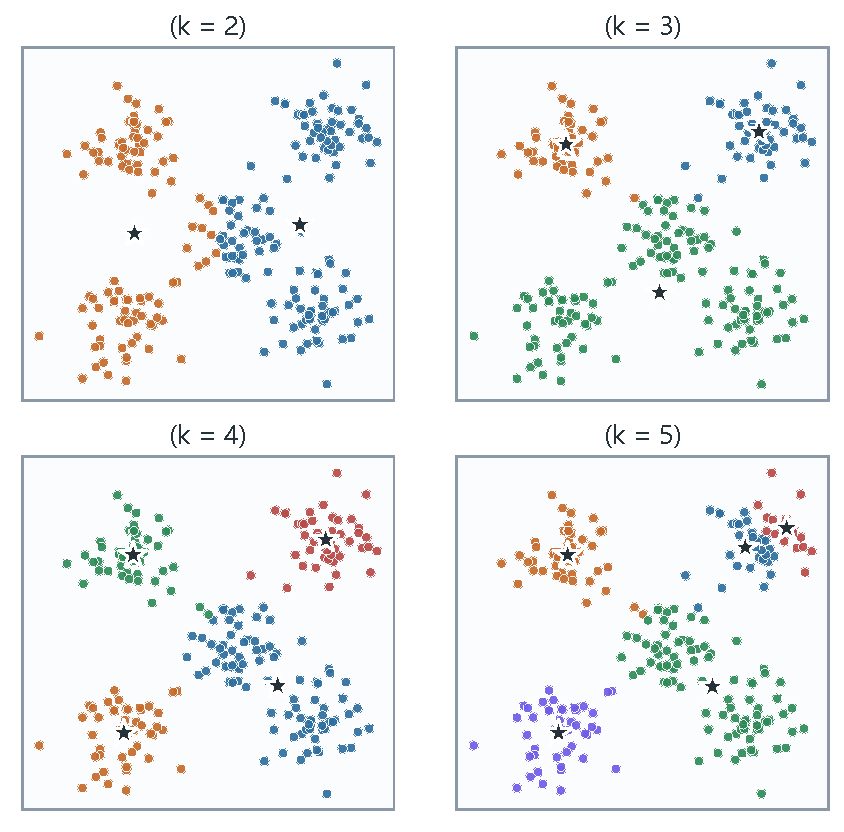
\includegraphics[width=0.72\textwidth]{pic/K-Means聚类效果示意图.pdf}
	\caption{K-Means聚类效果示意图}
	\label{fig:K-Means聚类效果示意图}
\end{figure}
\subsection{DBSCAN聚类}
DBSCAN是一种基于密度的聚类方法，无需预先指定簇数量，能够识别非凸形状的簇并将低密度离群点标记为噪声，因而适合处理形状不规则且含测量噪声的障碍物点云。其基本思想是通过密度可达关系连接高密度区域。对于数据集$D$中的任意点$p$，其$\varepsilon$邻域定义为
\begin{equation}
    N_{\varepsilon}(p)
    =\left\{q\in D\mid \operatorname{dist}(p,q)\leq\varepsilon\right\},
    \label{eq:dbscan_neighborhood}
\end{equation}
其中，$\varepsilon$为邻域半径，$\operatorname{dist}(\cdot)$为距离度量。若$\left|N_{\varepsilon}(p)\right|\geq \mathrm{MinPts}$，则$p$为核心点；位于某一核心点邻域内但自身不满足该条件的样本为边界点；既不是核心点、也不能由任何核心点密度可达的样本才被标记为噪声点。算法从未访问的核心点出发，将其邻域内所有密度可达的样本递归并入同一簇，直至无法继续扩展，再搜索下一个未访问的核心点。

DBSCAN的聚类效果主要受邻域半径$\varepsilon$和最小样本数$\mathrm{MinPts}$影响。$\varepsilon$过小时，同一障碍物的点云可能被分裂为多个簇；取值过大时，相邻障碍物可能被错误合并。$\mathrm{MinPts}$过小时，离群点容易形成伪簇；取值过大时，点云稀疏的真实障碍物可能被判为噪声。因此，两项参数需结合传感器分辨率、点云密度及目标距离进行设置。

在移动机器人环境感知中，DBSCAN可对激光雷达或深度相机点云进行聚类，并从各点簇提取障碍物边界与包围盒。图~\ref{fig:聚类效果对比示意图}展示了DBSCAN与K-Means处理非凸数据集时的聚类效果差异。
\begin{figure}[!htb]
    \centering
    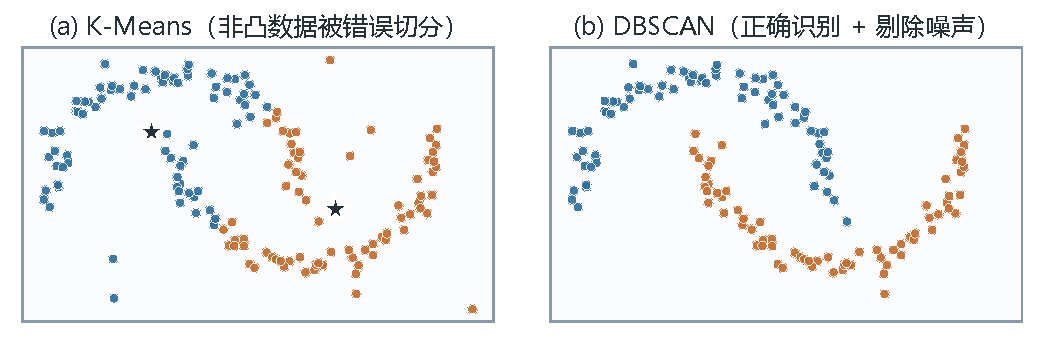
\includegraphics[width=0.92\textwidth]{pic/聚类效果对比示意图.pdf}
    \caption{聚类效果对比示意图}
    \label{fig:聚类效果对比示意图}
  \end{figure}

综合两种算法的特性可以看出，障碍物点云通常呈现任意形状、且不可预知簇数量、并伴随传感器噪声，这与DBSCAN算法所擅长处理的场景高度契合：它既无需预设障碍物数量，又能将离群噪声点自动剔除。因此，本章后续的点云检测器选用DBSCAN算法作为聚类内核，其检测流程将在下一节的障碍物检测跟踪系统中详细展开。

\section{障碍物检测跟踪系统}
受传感器配置与机载算力限制，移动机器人需要兼顾检测精度与计算效率。为此，本章构建如图~\ref{fig:障碍物检测与跟踪框架}所示的轻量级检测跟踪框架，主要包括障碍物检测、动态识别、状态跟踪和局部地图更新四个模块。

检测模块根据实际传感器配置接收深度图像或激光雷达点云。输入深度图像时，U深度图检测器直接从图像中提取障碍物，同时将深度图转换为点云并送入DBSCAN检测器；输入激光雷达点云时，则在裁剪与滤波后直接执行DBSCAN聚类。两个检测器输出的障碍物包围盒经过关联与融合后，由识别模块结合历史状态划分为静态目标和动态目标；跟踪模块完成跨帧数据关联并估计障碍物的运动状态；最后，地图更新模块将融合点云、障碍物边界及跟踪结果写入局部占用地图，为下游规划器提供环境约束。

\begin{figure}[!htb]
	\centering
	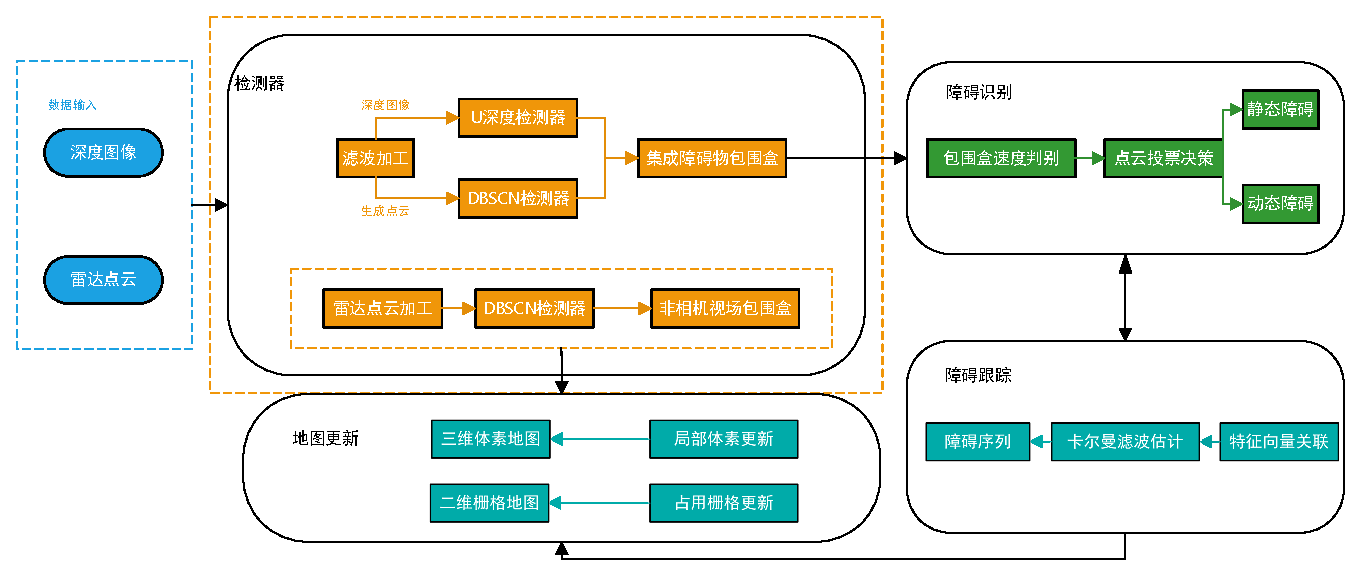
\includegraphics[width=\textwidth]{pic/检测流程.eps}
	\caption{障碍物检测与跟踪框架}
	\label{fig:障碍物检测与跟踪框架}
\end{figure}


\subsection{三维障碍物检测器}
环境检测由U深度图检测器与DBSCAN检测器组成。二者均采用非学习式方法，无需配置高算力推理硬件，适合部署于中小型移动机器人。U深度图检测器直接处理深度图像，DBSCAN检测器则处理由深度图反投影或由激光雷达获取的点云，两者对传感器噪声的敏感方式不同，可通过结果融合提高检测稳定性。

\textbf{（1）U深度图检测器。}U深度图方法已用于杂乱动态环境中的微型无人机避障\textsuperscript{\cite{7138979}}和拥挤室内环境中的动态目标检测\textsuperscript{\cite{10323166}}。该检测器通过三个步骤提取障碍物的三维轴对齐包围盒：生成U深度图、在U深度图中执行线段分组，以及在原始深度图中进行深度连续性搜索。

图~\ref{fig:检测器检测示意图}（a）和图~\ref{fig:检测器检测示意图}（b）分别为原始深度图像和U深度图像。系统按图像列统计深度值直方图生成U深度图，其横轴与原深度图像的列方向一致，纵轴表示离散深度区间。对U深度图中的连续区域进行分组，可得到图~\ref{fig:检测器检测示意图}（d）所示宽度为$w$、深度方向厚度为$t$的二维边界框；随后在原始深度图的对应列范围内执行深度连续性搜索，获得图~\ref{fig:检测器检测示意图}（a）所示的障碍物高度$h$。结合相机内参和深度值，即可将图像边界反投影至相机坐标系，再通过TF变换获得地图坐标系下障碍物的位置与三维尺寸。
\begin{figure}[!htb]
	\centering
	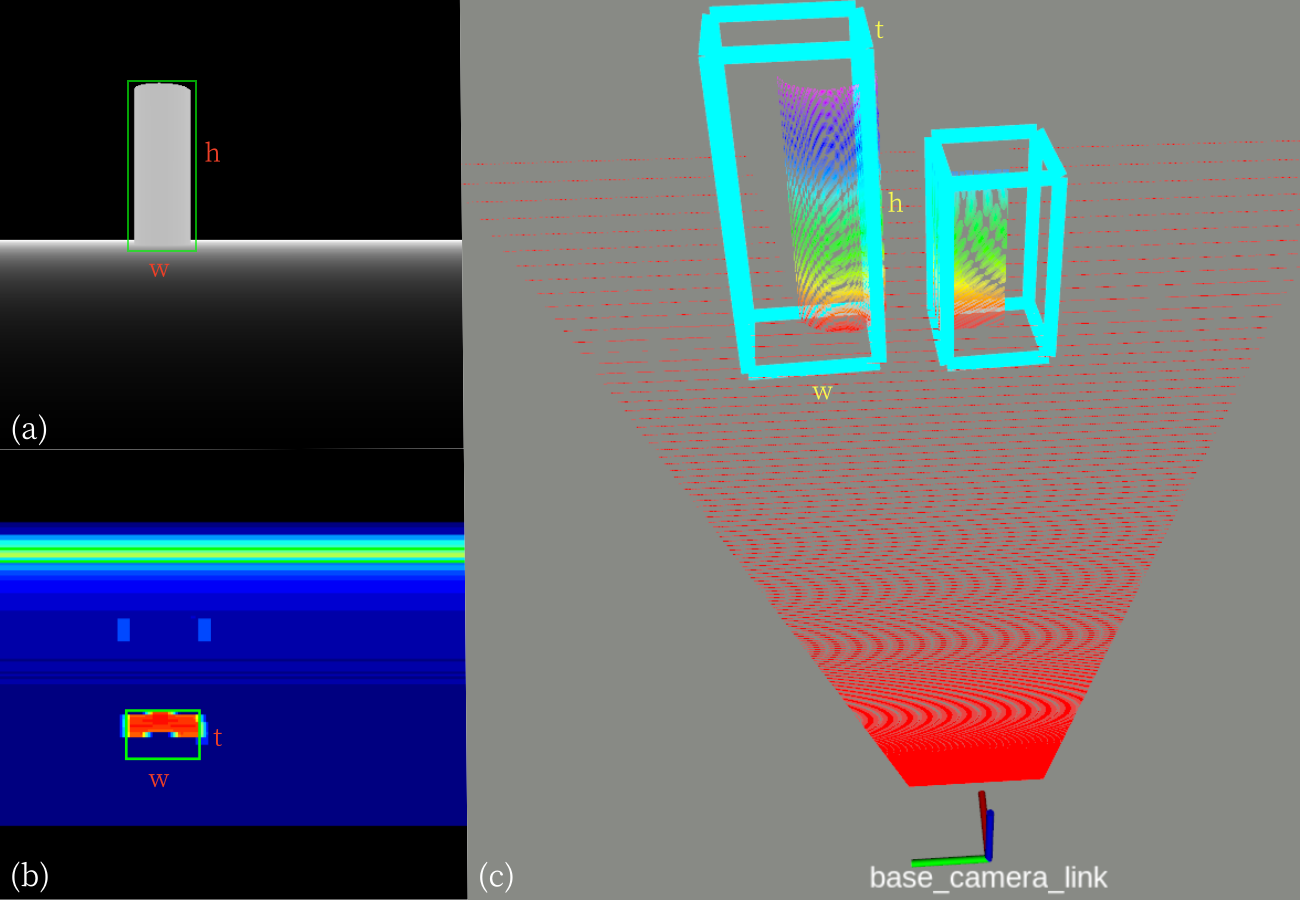
\includegraphics[width=0.85\textwidth]{pic/检测器检测示意图.png}
	\caption{检测器检测示意图}
	\label{fig:检测器检测示意图}
\end{figure}

\textbf{（2）DBSCAN检测器。}与基于图像的检测器不同，DBSCAN检测器直接处理点云数据。输入深度图像时，系统按第~\ref{sec:depth2cloud}节的方法将有效深度像素反投影为空间点；输入激光雷达点云时，则直接执行感兴趣区域裁剪。点云首先经过体素降采样和离群点过滤，再按第~\ref{sec:clustering}节所述DBSCAN方法聚类。对每个有效点簇分别计算最小、最大坐标，即可获得图~\ref{fig:检测器检测示意图}（c）所示的轴对齐包围盒。该检测器无需训练数据，且计算开销相对较低。

两个检测器并行运行并分别输出障碍物包围盒。由于深度图直方图与三维点云聚类具有不同的误差来源，同一真实障碍物通常会在两路结果中形成空间重叠，而单路噪声产生的伪检测往往缺少另一检测器的支持。因此，本文通过双向交并比（Intersection over Union, IoU）校验寻找两类结果中的一致检测，并采用保守策略融合相匹配的包围盒，以降低噪声对目标位置与尺寸估计的影响。

算法~\ref{alg:集成检测算法}给出了成对融合流程。对于检测器1输出的每个包围盒$b_{d1}$，先在检测器2的序列$B_{d2}$中搜索IoU最大的候选$b_{match1}$，再由$b_{match1}$反向搜索$B_{d1}$中的最佳匹配$b_{match2}$。仅当$b_{match2}=b_{d1}$且双向IoU均不低于阈值$S_{thr}$时，才将两者判定为互为最佳匹配。融合包围盒的中心取两者中心的平均值，各方向尺寸取两者对应尺寸的较大值，以避免低估障碍物范围。对于未通过匹配校验的检测结果，系统保留其原始包围盒，由后续跨帧跟踪进一步判断其有效性。

\begin{algorithm}[H]
    \KwIn{检测器1障碍物包围盒序列$B_{d1}$，检测器2障碍物包围盒序列$B_{d2}$，最小交并比阈值$S_{thr}$}
    \KwOut{集成包围盒序列$B_{en}$} 
    初始化$B_{en} \gets \emptyset$\;
    
    \For{$b_{d1} \in B_{d1}$}{
        $S_{iou1}, b_{match1} \gets \text{findBestIOUMatch}(b_{d1}, B_{d2})$\tcp{找到最佳匹配盒} 
        $S_{iou2}, b_{match2} \gets \text{findBestIOUMatch}(b_{match1}, B_{d1})$\tcp{反向验证匹配} 
        $flag \gets  (b_{match2} == b_{d1})$\; 
        
        \eIf{
            $S_{iou1} \geq S_{thr} \, \text{\normalfont\bfseries and} \, S_{iou2} \geq S_{thr} \, \text{\normalfont\bfseries and} \, flag$
        }{
            $b_{en} \gets \text{fuseBoxes}(b_{d1}, b_{match1})$\tcp{融合包围盒}
            $B_{en} \gets B_{en} \cup \{ b_{en} \}$\; 
        }{
            $B_{en} \gets B_{en} \cup \{ b_{d1} \}$\tcp{保留独立检测结果}
        }
    }
    返回$B_{en}$\;
    \caption{集成检测算法}
    \label{alg:集成检测算法}
\end{algorithm}

\subsection{障碍物关联跟踪}
当前帧检测得到的障碍物包围盒需与历史轨迹进行关联，以建立连续的目标身份并估计运动状态。本文采用基于特征相似度的匈牙利算法完成全局一一匹配\textsuperscript{\cite{JCDL202503143}}。与仅使用包围盒中心距离相比，联合考虑目标位置、尺寸和点云分布能够降低相邻动静态目标之间的错误关联概率。

深度相机可能因图像丢帧、目标遮挡或目标暂时离开视场而产生短时漏检。如图~\ref{fig:动态障碍物遮挡示意图}所示，机器人在前一时刻检测到墙后运动目标并生成避障轨迹；当目标短暂离开视场后，若立即删除其历史状态，规划器可能沿原路径继续运动，并在目标再次出现时来不及完成避让。为此，本文保留暂时失配目标的轨迹，并利用恒加速度模型在设定的最大丢失帧数内传播其状态；若后续观测重新匹配，则以新观测校正预测状态，否则在超过保留时限后删除该轨迹。该机制用于补偿短时观测中断，但预测不确定性会随失配时间增加，因此不能无限期保留外推结果。
\begin{figure}[!htb]
	\centering
	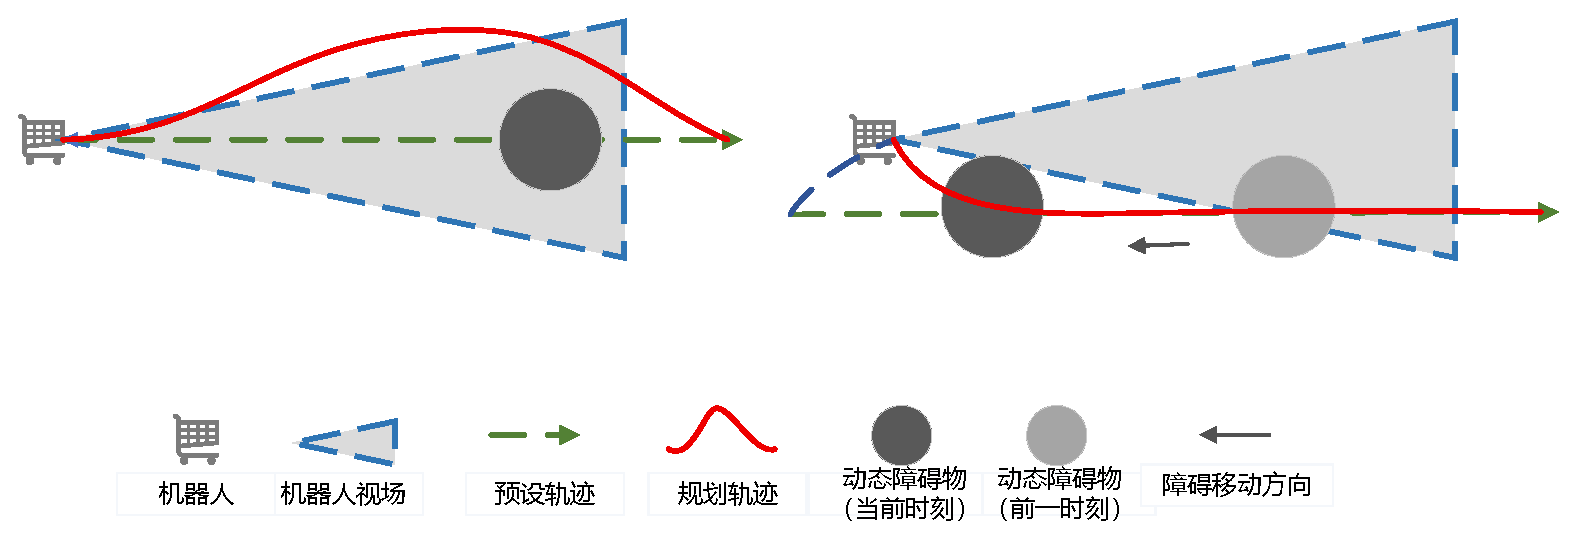
\includegraphics[width=1.0\textwidth]{pic/动态障碍物遮挡.eps}
	\caption{动态障碍物遮挡示意图}
	\label{fig:动态障碍物遮挡示意图}
\end{figure}

设第$i$个障碍物的归一化特征向量为
\begin{equation}
    \mathbf{f}(O_i)
    =\left[\mathbf{p}_i^{\mathrm{T}},\mathbf{d}_i^{\mathrm{T}},n_i,
    \boldsymbol{\sigma}_i^{\mathrm{T}}\right]^{\mathrm{T}},
    \label{eq:obstacle_feature}
\end{equation}
其中，$\mathbf{p}_i$为包围盒中心坐标，$\mathbf{d}_i$为包围盒在$x$、$y$、$z$方向上的尺寸，$n_i$为点簇所含点数，$\boldsymbol{\sigma}_i$为点簇坐标的标准差。各维特征按其统计尺度归一化后，定义障碍物$O_i$与$O_j$的相似度为
\begin{equation}
    s_{ij}
    =\exp\!\left(-\left\|\mathbf{f}(O_i)-\mathbf{f}(O_j)\right\|_2^2\right).
    \label{eq:obstacle_similarity}
\end{equation}
该函数将特征距离映射至$(0,1]$：距离越小，相似度越高。以$1-s_{ij}$构造关联代价矩阵，并通过匈牙利算法获得当前检测与历史轨迹之间的最小总代价匹配。为避免强制关联差异过大的目标，仅保留满足$s_{ij}\geq T_{sim}$的匹配对；未匹配检测用于初始化新轨迹，未匹配历史轨迹则进入短时预测保持状态。

障碍物完成数据关联后，采用二维恒加速度模型的卡尔曼滤波估计其运动状态。设地图坐标系下的状态向量为
\begin{equation}
    \mathbf{x}_t=[x_t,y_t,\dot{x}_t,\dot{y}_t,\ddot{x}_t,\ddot{y}_t]^{\mathrm{T}},
    \label{eq:ca_state}
\end{equation}
其中包含障碍物包围盒中心的二维位置、速度和加速度。采样间隔为$\Delta t$时，状态预测模型为
\begin{equation}
    \mathbf{x}_{t|t-1}=F\mathbf{x}_{t-1|t-1}+\mathbf{w}_t,
    \qquad \mathbf{w}_t\sim\mathcal{N}(\mathbf{0},Q),
    \label{eq:ca_prediction}
\end{equation}
其中
\begin{equation}
    F=\begin{bmatrix}
        1&0&\Delta t&0&\frac{1}{2}\Delta t^2&0\\
        0&1&0&\Delta t&0&\frac{1}{2}\Delta t^2\\
        0&0&1&0&\Delta t&0\\
        0&0&0&1&0&\Delta t\\
        0&0&0&0&1&0\\
        0&0&0&0&0&1
    \end{bmatrix}.
    \label{eq:ca_transition}
\end{equation}
若以零均值白噪声模拟模型未描述的平面加加速度，则可令$Q=GQ_jG^{\mathrm{T}}$，其中
\begin{equation}
    G=\begin{bmatrix}
        \Delta t^3/6&0\\0&\Delta t^3/6\\
        \Delta t^2/2&0\\0&\Delta t^2/2\\
        \Delta t&0\\0&\Delta t
    \end{bmatrix},\qquad Q_j=\sigma_j^2 I_2.
    \label{eq:ca_process_noise}
\end{equation}
参数$\sigma_j^2$表征真实目标运动偏离恒加速度假设的程度，其值越大，滤波器对新观测的响应越快，但状态估计的平滑性相应降低。

检测器直接观测的是包围盒中心位置，而非完整的六维运动状态。因此，观测模型写为
\begin{equation}
    \mathbf{z}_t=H\mathbf{x}_t+\mathbf{v}_t,
    \qquad \mathbf{v}_t\sim\mathcal{N}(\mathbf{0},R),
    \label{eq:ca_observation}
\end{equation}
\begin{equation}
    H=\begin{bmatrix}1&0&0&0&0&0\\0&1&0&0&0&0\end{bmatrix},
    \label{eq:ca_observation_matrix}
\end{equation}
其中，$R$为包围盒中心测量噪声协方差。卡尔曼滤波通过上述预测模型外推目标状态，并在获得新检测时利用位置观测完成校正；目标短时漏检时仅执行预测步骤，从而为视距外补偿提供连续的位置、速度与加速度估计。

\subsection{动态障碍物识别}
单独依据包围盒中心速度判断目标是否运动，容易将视场变化、包围盒尺寸抖动和关联误差造成的假位移误判为真实运动。为降低假阳性，本文采用“包围盒速度初筛—点云运动一致性复核”的两阶段判据：仅当包围盒中心速度超过阈值，且包围盒内足够比例的有效点与包围盒具有一致运动趋势时，才将目标标记为动态。对于连续多个历史帧均被判为动态的目标，采用有限时长的状态保持以避免短时漏检引起标签频繁切换。算法~\ref{alg:fusion1}给出了具体流程。

\begin{algorithm}[H]
	\caption{动态障碍物检测分类算法}
	\label{alg:fusion1}
	\SetAlgoLined
	\SetKw{Continue}{continue}
	\LinesNumbered
	\KwIn{目标障碍物列表$B_{tar}$，障碍物历史包围盒信息$BoxHist$，障碍物历史点云序列$PcHist$，强制执行帧数$forceFrame$，包围盒速度阈值$vbox_{th}$，点云速度阈值$vpc_{th}$，投票比例阈值$vote_{th}$}
    \KwOut{动态障碍物列表 $B_{dy}$} 
	
	\BlankLine
	$B_{dy} \leftarrow \emptyset$\;
	\For{$i \gets 0$ \KwTo $|B_{tar}|-1$} {
		$\texttt{DataAssociation}(B_{tar}[i], BoxHist)$ \tcp{关联当前包围盒与历史数据}
		$n \leftarrow |BoxHist[i]|$ \tcp{获取历史列表长度}
		\If{$\sum_{j=1}^{n} BoxHist[i][j].{is\_dynamic} \geq {forceFrame}$} 
		{
			$BoxHist[i][0].{is\_dynamic} \leftarrow {true}$\;
			$B_{dy}.{push\_back}(B_{tar}[i])$\tcp{添加到动态障碍物列表}
			\Continue\;	
		}
		${votes} \leftarrow 0$，$n_{valid}\leftarrow0$\tcp{初始化投票数与有效点数}
		$\mathbf{v}_{box}\leftarrow \left(\mathbf{P}_{box}(t)-\mathbf{P}_{box}(t-1)\right)/\Delta t$\;
		\ForEach{$p \in PcHist[i][0]$}{
			\If{$p$在$t-1$时刻存在有效对应点}{
				$n_{valid}\leftarrow n_{valid}+1$\;
				计算点速度$\mathbf{v}_{p}$\;
				\If{$\mathbf{v}_{p}^{\mathrm T}\mathbf{v}_{box}\geq0\;\&\&\;\|\mathbf{v}_{p}\|_2>vpc_{th}$}{
					$votes\leftarrow votes+1$\;
				}
			}
		}
		$r_{vote}\leftarrow votes/\max(n_{valid},1)$\;
		\If{$\|\mathbf{v}_{box}\|_2\geq vbox_{th}\;\&\&\;r_{vote}\geq vote_{th}$}{
			$B_{dy}.{push\_back}(B_{tar}[i])$\tcp{添加到动态障碍物列表}
		}
	}	
	返回$B_{dy}$\;
\end{algorithm}

算法首先将当前帧障碍物与历史轨迹关联，并检查对应轨迹的动态标签历史。若目标已连续多帧被判为动态，则在有限保持帧数内延续动态标签，以降低短时停顿或漏检造成的标签抖动。该滞回机制会延迟“运动转静止”的判定，因此保持帧数不宜过大。

对未触发标签保持的目标，包围盒中心速度由
\begin{equation}
    \mathbf{v}_{box}(t)
    =\frac{\mathbf{P}_{box}(t)-\mathbf{P}_{box}(t-1)}{\Delta t}
    \label{eq:bbox_velocity}
\end{equation}
计算。随后通过最近邻搜索建立当前点云与前一时刻点云之间的对应关系，并计算有效点速度$\mathbf{v}_p$。当$\mathbf{v}_p^{\mathrm T}\mathbf{v}_{box}\geq0$且$\|\mathbf{v}_p\|_2>vpc_{th}$时，该点为动态假设投一票。记有效对应点数为$n_{valid}$，则投票比例为$r_{vote}=votes/\max(n_{valid},1)$。仅当$\|\mathbf{v}_{box}\|_2\geq vbox_{th}$且$r_{vote}\geq vote_{th}$时，目标才被判为动态。

点云投票前还需剔除不具有跨帧对应关系的点。如图~\ref{fig:去除无效点云示意图}所示，机器人接近部分可见的静态障碍物时，视场扩大可能使包围盒中心由红色五角星位置移动至绿色五角星位置，从而产生较大的表观中心速度。当前帧中新出现的绿色点在前一帧不可见，无法形成可靠的速度观测；若将其计入投票，静态障碍物可能被误判为动态。因此，算法仅对两帧中均可见且匹配有效的点计算速度，并将新进入视场的点排除在投票集合之外。

\begin{figure}[!htb]
	\centering
	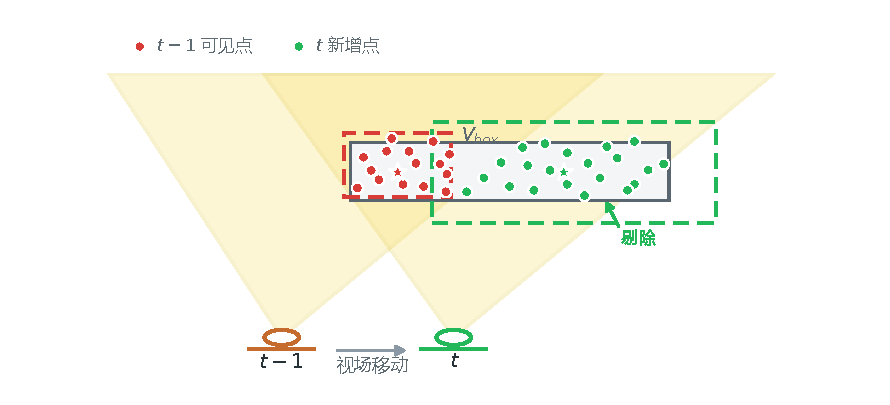
\includegraphics[width=1.0\textwidth]{pic/去除无效点云示意图.pdf}
	\caption{去除无效点云示意图}
	\label{fig:去除无效点云示意图}
\end{figure}

\section{局部地图构建策略}
本节与第2章的传感器级点云融合承担不同功能：第2章将激光雷达与深度相机观测统一到$\mathrm{base\_link}$坐标系，并发布去噪后的融合点云$\mathrm{/local\_pointcloud}$；本节以该点云以及障碍物检测、关联跟踪和动态状态识别结果为输入，构造直接服务于规划安全约束的局部占用地图。

系统首先结合同步位姿，将融合点云中的有效障碍点和包围盒边界点变换至地图坐标系；随后通过射线更新记录已观测自由空间与障碍占用，并在占用层上执行安全膨胀。输入观测与定位信息采用近似时间同步，以减小机器人运动造成的时空错位。为适应动态或半静态环境，系统同时维护局部更新窗口，使暂态误检和长期未被观测确认的陈旧占用能够被后续自由空间观测清除。

对于每个有效量测点，构造从传感器光心到量测端点的射线，并采用Bresenham算法\textsuperscript{\cite{9702849}}遍历射线覆盖的栅格单元。射线沿途单元记为自由，终端单元记为占用。设栅格$v$在时刻$t$的占用概率为$p_t(v)$，其对数几率表示为
\begin{equation}
    L_t(v)=\log\frac{p_t(v)}{1-p_t(v)}.
    \label{eq:local_map_logodds}
\end{equation}
使用对数几率后，多帧观测可通过增量累加完成融合。令自由观测增量$l_{free}<0$，占用命中增量$l_{occ}>0$，则栅格状态递推为
\begin{equation}
    L_t(v)=\operatorname{clip}\!\left(L_{t-1}(v)+\Delta L(v),L_{\min},L_{\max}\right),
    \label{eq:local_map_update}
\end{equation}
其中
\begin{equation}
    \Delta L(v)=
    \begin{cases}
        l_{free}, & v\in R_f,\\
        l_{occ},  & v=R_{end}.
    \end{cases}
    \label{eq:local_map_inverse_sensor}
\end{equation}
式中，$\operatorname{clip}(\cdot)$将对数几率限制在$[L_{\min},L_{\max}]$内，以避免重复观测造成数值饱和；$R_f$为射线沿途的自由栅格集合，$R_{end}$为射线终端栅格。连续自由观测可逐步降低陈旧占用的对数几率，从而释放已确认无障碍的空间。

为将机器人几何尺寸以及定位与控制误差纳入安全约束，系统在占用图上执行形态学膨胀。记阈值化后的占用集合为
\begin{equation}
    \mathcal{O}=\left\{v\mid p(v)>\tau\right\},
    \label{eq:occupied_set}
\end{equation}
其中$\tau$为占用概率阈值。设膨胀半径为$r_{infl}$，则膨胀后的障碍集合定义为
\begin{equation}
    \mathcal{O}^{\oplus}
    =\left\{u\mid \exists v\in\mathcal{O},\ \|u-v\|_2\leq r_{infl}\right\}.
    \label{eq:inflated_obstacle_set}
\end{equation}
实现中对新近更新的局部地图周期性执行膨胀，并生成布尔化的膨胀占用掩膜。由此，系统既保留障碍物边界信息，也记录视线内的自由空间证据，为下游路径规划提供可直接查询的安全约束。

\section{本章小结}
本章面向资源受限移动机器人在复杂动态环境中的障碍感知需求，研究了障碍物检测、关联跟踪、动态识别与局部地图更新方法。首先介绍K-Means和DBSCAN聚类原理，结合障碍物点云形状不规则、簇数量未知且含离群噪声的特点，选用DBSCAN作为点云检测器的聚类内核。

随后，构建了由U深度图检测器与DBSCAN点云检测器组成的轻量级并行检测框架，并通过双向IoU校验和保守包围盒融合降低单一检测器的误检影响。在跨帧跟踪阶段，采用归一化位置、尺寸和点云分布特征构造关联代价，通过匈牙利算法获得一一匹配；针对短时遮挡与目标暂时离开视场的情况，利用恒加速度卡尔曼滤波传播目标状态，为规划器提供连续的位置、速度与加速度估计。

在动态障碍物识别方面，采用包围盒中心速度进行初筛，并利用跨帧有效点的运动一致性进行投票复核；通过投票比例判据和有限时长的动态标签保持，降低包围盒抖动、视场变化和短时漏检引起的误判。最后，以第2章输出的多传感器融合点云及本章检测跟踪结果为输入，采用Bresenham射线遍历和对数几率更新记录自由空间与障碍占用，并通过形态学膨胀生成安全边界。

本章向第5章局部规划器提供三类信息：DBSCAN聚类后的障碍边界点及AABB包围盒，动态障碍物的位置、速度与加速度估计，以及包含自由空间和安全膨胀结果的局部占用地图。这些输出为动态预测点流构造和神经距离编码MPC的点级几何约束提供了环境输入。
